\documentclass[12pt]{article}
\usepackage[russian]{babel}
\usepackage[utf8]{inputenc}
\inputencoding{utf8}
\usepackage{geometry}\geometry{a4paper, margin=2cm}
\usepackage[numbers,sort&compress,square]{natbib}
\usepackage{hyperref,xcolor}
\usepackage{graphicx,caption,subcaption}
\usepackage{indentfirst,amsmath,amssymb,textcomp}
\usepackage{url}
\usepackage{physics}
\sloppy
\title{Уравнение теплопроводности.}
\author{}
\date{}

\renewcommand{\vec}[1]{\textbf{#1}}
\newcommand{\task}[2]{\vspace{6pt}
\textbf{Задание #1}. #2 %\vspace{6pt}
}

\begin{document}
\maketitle

Дан металлический стержень длины $L$, теплоизолированный по всей длине за исключением двух концов. Стержень изначально имеет температуру $T_0$, допустим, $100^\circ \mathrm{C}$, а концы погружены в холодную среду, например, воду температуры $0^\circ \mathrm{C}$. Необходимо найти распределение температуры в стержне с течением времени.

Данная задача сводится к решению одномерного уравнения теплопроводности:
%
\begin{equation}
\frac{\partial T(x, t)}{\partial t}=a^2\frac{\partial^2 T(x, t)}{\partial^2 x},
\label{eq:heat}
\end{equation}
%
где $a^2=K/C\rho$, $K$ --- коэффициент теплопроводности, $C$ --- теплоёмкость, $\rho$ --- плотность материала. Это уравнение в частных производных параболического типа, и подразумевает как граничные, так и начальные условия, в нашем случае:
%
\begin{equation}
T(x,t=0)=100^\circ\mathrm{C},\quad T(x=0,t)=T(x=L,t)=0^\circ\mathrm{C}.
\end{equation}
Уравнение с такими граничными условиями можно решить аналитически методом разделения переменных. Однако предлагается решить это уравнение численно с помощью конечно-разностной схемы.

\section*{Явная схема}
\begin{figure}
\begin{center}
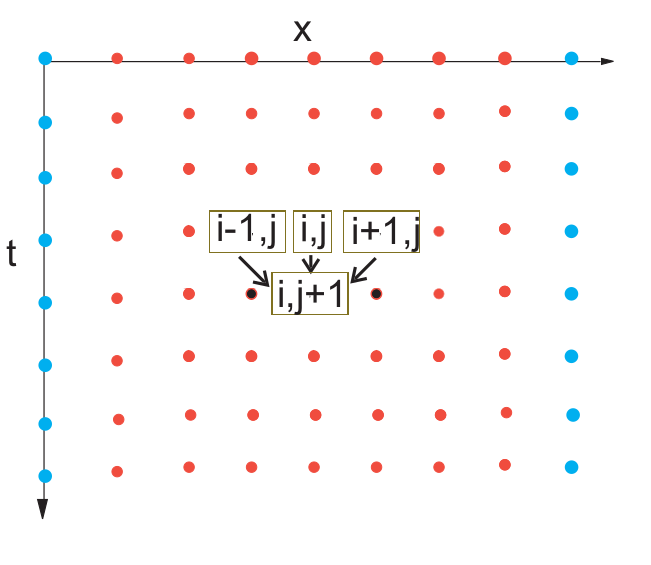
\includegraphics[width=0.6\linewidth]{./figs/01.png}
\caption{Явная схема решения уравнения теплопроводности.}
\label{fig:explicit}
\end{center}
\end{figure}
\begin{figure}
\begin{center}
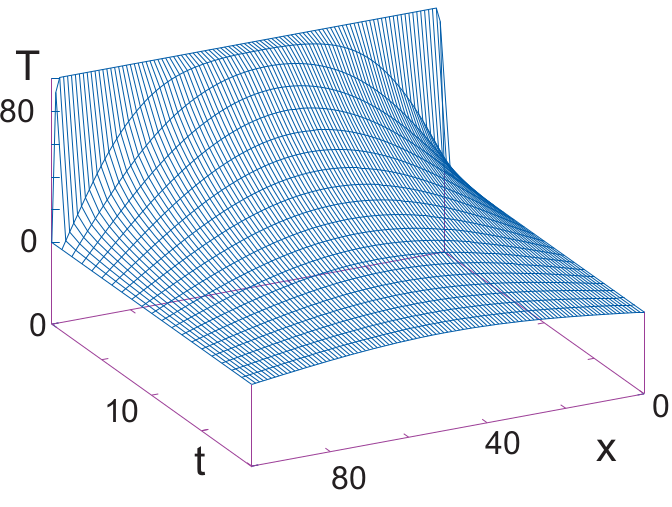
\includegraphics[width=0.6\linewidth]{./figs/02.png}
\caption{Эволюция распределения температуры в стержне.}
\label{fig:solution}
\end{center}
\end{figure}
Как обычно, конечно-разностная схема основывается на аппроксимации производных в уравнении на сетке с конечным шагом. Пространство и время дискретизуется с шагами $\Delta t$ и $\Delta x$, и ищется приближённое решение в узлах сетки (см. Рис. \ref{fig:explicit}). Производные можно заменять на приближённые не единственным способом, что приводит к разным вариантам схем. Самый простой (но не самый лучший) вариант --- \textit{явная схема}. Так как значения температуры на сетке при $t=0$ известны, производная по времени выражается как
%
\begin{equation}
\frac{\partial T(x, t)}{\partial t}\approx \frac{T(x,t+\Delta t)-T(x,t)}{\Delta t},
\end{equation}
%
которую также называют \textit{правой односторонней производной}. Так как известно значение температуры на краях стержня, для второй производной по времени можно использовать аппроксимацию:
%
\begin{equation}
\frac{\partial^2 T(x, t)}{\partial^2 x}\approx \frac{T(x+\Delta x,t)-2T(x,t)+T(x-\Delta x, t)}{(\Delta x)^2}.
\end{equation}
После подстановки аппроксимаций в уравнение \eqref{eq:heat} его переписать в виде:
%
\begin{equation}
T_{i,j+1}=T_{i,j}+\eta\left[T_{i+1,j}+T_{i-1,j}-T_{i,j}\right], \quad \eta=\frac{a^2 \Delta t}{\Delta x^2},
\end{equation}
%
где $x=i\Delta x$, $t=j\Delta t$, $i=\overline{0,N}$, $j=0,1,2,\ldots$. Такая схема называется \textit{явной}, потому что она позволяет выразить решение через известные значения температуры. Начиная с верхнего ряда по $j$ (см. Рис. \ref{fig:explicit}), можно вычислить, как меняется распределение температуры в стержне со временем, как, например, показано на Рис. \ref{fig:solution}.

Во время решения уравнения в частных производных с помощью разностных методов нужно помнить о \textit{сходимости схемы} к точному решению. Можно показать, что явная схема сходится, только если выполнено условие:
%
\begin{equation}
\eta=\frac{a^2\Delta t}{\Delta x^2}<\frac{1}{2}.
\label{eq:stability}
\end{equation}
%
Из этого условия вытекает, что выбор сеток по времени и пространству не произволен. С уменьшением шага по времени $\Delta t$ сходимость всегда улучшается, но если по каким-то причинам нужно найти более детальное решение по пространству, необходимо уменьшить шаг $\Delta t$ причём пропорционально $\Delta x^2$! Это является одним из главных недостатков явных схем решений уравнений в частных производных в целом. Отсутствие сходимости к решению (например, при нарушении условия \eqref{eq:stability} в случае уравнения теплопроводности) может проявляться как бесконечный рост численного решения со временем или через быстрый рост высокочастотных гармоник, которые никак не связаны с физической природой изучаемого процесса.

\section*{Неявная схема Кранка-Николсона}
Метод Кранка-Николсона позволяет находить решение уравнения теплопроводности \eqref{eq:heat} со значительно большей точностью. Суть метода заключается в альтернативном способе аппроксимации производных в уравнении. Вместо правой односторонней производной по времени будем использовать \textit{центральную производную}:
%
\begin{equation}
\frac{\partial T}{\partial t}\left(x,t+\frac{\Delta t}{2}\right)\approx \frac{T(x,t+\Delta t)-T(x,t)}{\Delta t}+O(\Delta t^2),
\end{equation}
%
а вторую производную по времени в момент $t+\frac{\Delta t}{2}$ выразим как
%
\begin{equation}
\begin{split}
2(\Delta x)^2\frac{\partial^2 T}{\partial^2 x}\left(x,t+\frac{\Delta t}{2}\right)\approx & \left[T(x+\Delta x,t+\Delta t)-2T(x,t+\Delta t)+T(x-\Delta x, t+\Delta t)\right]\\
& + \left[T(x+\Delta x,t)-2T(x,t)+T(x-\Delta x, t)\right]+O(\Delta x^2).
\end{split}
\end{equation}
%
Тогда уравнение теплопроводности аппроксимируется схемой
%
\begin{equation}
T_{i,j+1}-T_{i,j}=\frac{\eta}{2}\left(T_{i-1,j+1}-2T_{i,j+1}+T_{i+1,j+1}+T_{i-1,j}-2T_{i,j}+T_{i+1,j}\right).
\end{equation}
%
Видно, что теперь в уравнении перепутаны <<старые>> ($j+1$) и <<новые>> ($j+1$) значения температуры в узлах $i-1,\,i,\,i+1$, поэтому невозможно явно выразить <<новые>> значения температуры через <<старые>>, и получить решение, последовательно обходя сетку. Полученное уравнение по является матричным, и его необходимо решать целиком. Для этого уравнение переписывают в виде
%
\begin{equation}
-T_{i-1,j+1}+\left(\frac{2}{\eta}+2\right)T_{i,j+1}-T_{i+1,j+1}=-T_{i-1,j}+\left(\frac{2}{\eta}+2\right)T_{i,j}-T_{i+1,j}.
\end{equation}
%
Это уравнение позволяет \textit{неявно} найти $T_{i,j+1}$ для всех $i=\overline{0,N}$ сразу. Его можно записать в трёх-диагональном виде:
%
\begin{equation}
\begin{array}{c}
\begin{pmatrix}
\left(\frac{2}{\eta}+2\right) & -1 & \hphantom{1} & \hphantom{1} & \hphantom{1} & \hphantom{1}\\
-1 & \left(\frac{2}{\eta}+2\right) & -1 & \hphantom{1} & \hphantom{1} & \hphantom{1}\\
\hphantom{1} & -1 & \left(\frac{2}{\eta}+2\right) & -1 & \hphantom{1} & \hphantom{1}\\
\hphantom{1} & \hphantom{1} & \ddots & \ddots & \ddots & \hphantom{1}\\
\hphantom{1} & \hphantom{1} & \hphantom{1} & -1 & \left(\frac{2}{\eta}+2\right) & -1\\
\hphantom{1} & \hphantom{1} & \hphantom{1} & \hphantom{1} & -1 & \left(\frac{2}{\eta}+2\right)\\
\end{pmatrix}
\begin{pmatrix}
\vphantom{\left(\frac{2}{\eta}\right)} T_{1,j+1}\\
\vphantom{\left(\frac{2}{\eta}\right)} T_{2,j+1}\\
\vphantom{\left(\frac{2}{\eta}\right)} T_{3,j+1}\\
\vphantom{\left(\frac{2}{\eta}\right)} \vdots\\
\vphantom{\left(\frac{2}{\eta}\right)} T_{N-2,j+1}\\
\vphantom{\left(\frac{2}{\eta}\right)} T_{N-1,j+1}
\end{pmatrix}=\\
\hphantom{1111}\\
=\begin{pmatrix}
T_{0,j+1}+T_{0,j}-\left(\frac{2}{\eta}+2\right)T_{1,j}+T_{2,j}\\
T_{1,j}-\left(\frac{2}{\eta}+2\right)T_{2,j}+T_{3,j}\\
T_{2,j}-\left(\frac{2}{\eta}+2\right)T_{3,j}+T_{4,j}
\vphantom{\left(\frac{2}{\eta}\right)} \vdots\\
T_{N-3,j}-\left(\frac{2}{\eta}+2\right)T_{N-2,j}+T_{N-1,j}\\
T_{N-2,j}-\left(\frac{2}{\eta}+2\right)T_{N-1,j}+T_{N,j}+T_{N,j+1}
\end{pmatrix}.
\end{array}
\label{eq:matrix}
\end{equation}
%
Стартуя с начальных условий $T_{i,0}$, можно последовательно находить распределение температуры в стержне в последующие моменты времени, на каждом шаге по $j$ решая матричное уравнение \eqref{eq:matrix}. Так как матрица является трёх-диагональной, его можно эффективно решить, например, \textit{методом прогонки} \url{https://ru.wikipedia.org/wiki/%D0%9C%D0%B5%D1%82%D0%BE%D0%B4_%D0%BF%D1%80%D0%BE%D0%B3%D0%BE%D0%BD%D0%BA%D0%B8}.

Метод Кранка-Николсона устойчив для любых значений $\Delta t$ и $\Delta x$, и поэтому позволяет находить более точное решение по координатам, не слишком уменьшая при этом шаг по времени.


\section*{Задание}

\task{1}{\textit{(3 баллa)}} Найдите аналитическое решение задачи о температуре в стержне, поставленной в самом начале. Постройте решение в виде температурной карты или поверхности в пространстве $(x,t)$.

\task{2}{\textit{(баллa)}} Напишите программу, реализующую явную схему решения уравнения теплопроводности и решите поставленную задачу со стержнем (размер сетки по пространству порядка 100, по времени --- 500).
\begin{itemize}
\item Постройте решение $T(x)$ на одном графике в различные моменты времени.
\item Постройте решение $T(t)$ на одном графике для различных значений координат.
\item Сравните с точным решением.
\item Постройте изотермы (линии постоянной температуры).
\item Изучите сходимость схемы, посмотрите, что будет, если нарушить условие \eqref{eq:stability}.
\item Пусть теперь начальное условие задаётся законом $T(x,0)=\sin(\pi x/L)$. Найдите решение.
\end{itemize}

\task{3}{\textit{(баллa)}} Реализуйте метод Кранка-Николсона (неявная схема). Для этого изучите, как решать матричные уравнения методом прогонки и реализуйте его. Решите первоначальную задачу со стержнем (размер сетки по пространству порядка 100, по времени --- 100).
\begin{itemize}
\item Постройте графики для $T(x)$, $T(t)$, сравните их с полученными в задании 2.
\item Сравните явную и неявную схемы с точки зрения точности и скорости работы.
\end{itemize}

\task{4}{\textit{(баллa)}} Решите 2 следующие задачи:
\begin{itemize}
\item Пусть есть 2 стержня, соприкасающиеся торцами, и изначально температура одного из них равна $50^\circ \mathrm{C}$, а второго $100^\circ \mathrm{C}$. Свободные концы стержней держат при $0^\circ \mathrm{C}$. Постройте распределение температуры в пространстве $(x,t)$.
\item \textbf{Охлаждение Ньютона}. Предположим, что стержень помещён не в теплоизолирующий материал, а в среду с температурой $T_e$. Закон охлаждения Ньютона гласит:
\[\frac{\partial T}{\partial t}=-h(T-T_e),\]
где $h$ --- неотрицательная константа. Это приводит к изменению уравнения теплопроводности:
\[\frac{\partial T(x, t)}{\partial t}=a^2\frac{\partial^2 T(x, t)}{\partial^2 x}-h(T-T_e).\]
Измените одну из описанных схем и решите задачи с одним и двумя соприкасающимися стержнями.
\end{itemize}
\end{document}
